% TODO L, clust, cent,...-re (bővebb listát lásd az explor...ipynb): 
%   irányított más-e, súlyozott más-e, 
%   mekkorára tudom kiszámolni
% koncepció: mindn csak ötlet és illusztráció, minimális pilot redmény (a
% closeness cent és a HITS) 

\documentclass{beamer}
\usepackage[size=a0,debug]{beamerposter}

\usepackage{graphicx}			% allows us to import images
\usepackage{booktabs}
%\usepackage{amsmath}
%\usepackage{multirow}
\usepackage[utf8]{inputenc}
\usepackage{t1enc}
%\usepackage{anyfontsize}
%\usepackage{authordate1-4}
%%\usepackage{multirow}
\usetheme{cpbgposter}
\usepackage[round]{natbib}
%\usepackage{tikz}
\usepackage{url}
%\usepackage[magyar]{babel} TODO

%%%%%%%%%%%%%%%%%%%%%%%%%%%%%%%%%%%%%%%%%%%%%%%%%%%%%%%%%
% Define the column width and poster size
% To set effective sepwid, onecolwid and twocolwid values, first choose how
% many columns you want and how much separation you want between columns
% The separation I chose is 0.024 and I want 4 columns
% Then set onecolwid to be (1-(4+1)*0.024)/4 = 0.22
% Set twocolwid to be 2*onecolwid + sepwid = 0.464
%%%%%%%%%%%%%%%%%%%%%%%%%%%%%%%%%%%%%%%%%%%%%%%%%%%%%%%%%

\newlength{\sepwid}
\newlength{\onecolwid}
\newlength{\twocolwid}
\setlength{\paperwidth}{48in} % hogy ne lógjon rá az utolsó oszlop a keretre
%\setlength{\paperheight}{36in}
\setlength{\sepwid}{0.024\paperwidth}
\setlength{\onecolwid}{0.22\paperwidth}
\setlength{\twocolwid}{0.464\paperwidth}
%\setlength{\topmargin}{-0.5in}
%\usetheme{confposter}
%\usepackage{exscale} % scaling of the math extension font cmex

%%%%%%%%%%%%%%%%%%%%%%%%%%%%%%%%%%%%%%%%%%%%%%%%%%%%%%%%
% The next part fixes a problem with figure numbering. Thanks Nishan!
% When including a figure in your poster, be sure that the commands are typed in the following order:
% \begin{figure}
% \includegraphics[...]{...}
% \caption{...}
% \end{figure}
% That is, put the \caption after the \includegraphics
%%%%%%%%%%%%%%%%%%%%%%%%%%%%%%%%%%%%%%%%%%%%%%%%%%%%%%%%%

\usecaptiontemplate{
  \small
  \structure{\insertcaptionname~\insertcaptionnumber:}
\insertcaption}

% Define colours (see beamerthemeconfposter.sty to change these colour
% definitions) TODO

\setbeamercolor{block title}{fg=dblue,bg=white}
\setbeamercolor{block body}{fg=black,bg=white}
\setbeamercolor{alerted title}{fg=white,bg=dblue}
\setbeamercolor{block alerted title}{fg=white,bg=dblue!70}
\setbeamercolor{block alerted body}{fg=black,bg=dblue!10}
\setbeamercolor{alerted text}{fg=dgreen}
\setbeamercolor{item}{fg=dgreen}
\setbeamercolor{item projected}{bg=dgreen}

\author{Makrai Márton és Sass Bálint}
\title{A szöveg mint skálafüggetlen hálózat}
\institute{MTA Nyelvtudományi Intézet\break
{\tt \{makrai.marton,sass.balint\}@nytud.mta.hu}}

\begin{document}

\addtobeamertemplate{headline}{}
{
  \begin{tikzpicture}[remember picture,overlay]
    \node [shift={(-10 cm,-4cm)}]
    at (current page.north east)
    {\includegraphics[height=5cm]{/home/makrai/repo/paper/Common/Logo/nytud/logo_only_tr.png}};
  \end{tikzpicture}
}

\begin{frame}[t]
  \begin{columns}[t]% the [t] option aligns the column's content at the top
    % TODO Data, repo

    \begin{column}{\sepwid}\end{column}			% empty spacer column

    \begin{column}{\onecolwid} % bal oszlop
      \begin{block}{Hatványeloszlás, szavak, élek}
        \begin{itemize}
          \item szógyakoriságok \cite{Zipf:1935}
          \item skálafüggetlen gráf \citep{barabasi1999emergence}
          \item most: irányított gráf súlyozott élekkel bigramgyakorliságokból
        \end{itemize}

        \begin{figure}[ht]
          \begin{center}
            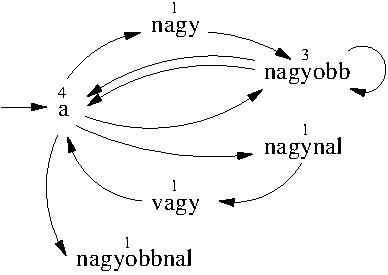
\includegraphics[width=.6\columnwidth]{scfr_pelda.pdf}
          \end{center}
            \caption{,,A nagyobb nagyobb a nagynál vagy a nagy nagyobb a nagyobbnál.''
            példamondat ábrázolása.
            A dupla nyilat ábrázolhatjuk egy 2-es súllyal bíró szimpla nyíllal is.}
            \label{fig:scfr_pelda}
        \end{figure}
      \end{block}

      %\smallskip

      \begin{block}{Kapcsolódó irodalom}
        \begin{itemize}
          \item TextRank \citep{mihalcea2004textrank}, kulcsszókinyerés
            \begin{quote}
              results [...] are worse than results obtained with undirected
                graphs, which suggests that [...] there is no natural “direction”
            \end{quote}
          \item szemantikus hálók \citep{steyvers2005large}
          \item trigram \citep{cancho2001thesmall}
          \item a skálafüggetlen-hipe kritikája
            \citep{willinger2009mathematics}
        \end{itemize}
      \end{block}
      
      %\begin{block}{Skálafüggetlenség}\end{block}

        \begin{alertblock}{Irányított kisvilág}  \end{alertblock} 
        \begin{block}{Utak, tranzitivitás} 
      \begin{table}
      \begin{tabular}{rrrrrrr}
        %TODO L, tranz: kell irányítatlan?
        \toprule
        mondat & szókincs & bigram & \multicolumn{2}{c}{$L$} & \multicolumn{2}{c}{tranzitivitás} \\
        &&&$\rightarrow$&--&$\rightarrow$&--\\
        \midrule
        10 & 125 & 165 & 7.02 & 4.19 & 0.02086 & 0.007463 \\
        100 & 880 & 1343 & 6.00 & 3.97 & 0.008146 & 0.004343 \\
        1k & 6828 & 12952 & 4.89 & 3.50 & 0.004051 & 0.00263 \\ 
        10 k	&     42 992  &     111 141 & 4.11 && 0.002058 & 0.001713 \\
        100 k	&    225 481  &     865 512 & \\
        1 m	  &  1 043 583  &   6 082 994 \\
        10 m	&  4 444 502  &  38 167 116 \\
        47 m  & 11 245 533  & 119 857 666 \\
        \bottomrule
      \end{tabular}
      \end{table}
          \begin{itemize}
            \item MNSZ2 \citep{oravecz2014hungarian}
          \end{itemize}
        \end{block}

          \begin{block}{Irányított klaszterezési együttható \citep{fagiolo2007clustering}}
            \begin{figure}
              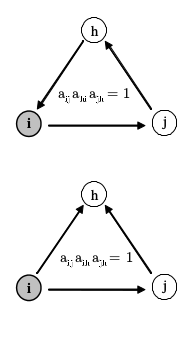
\includegraphics[width=7.5cm]{triangle-directions_1}
              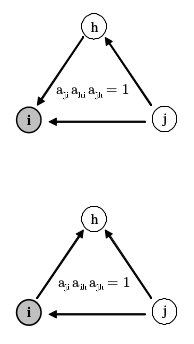
\includegraphics[width=7.5cm]{triangle-directions_2}
            \end{figure}
          \end{block}
    \end{column}

    \begin{column}{\sepwid} \end{column}			% empty spacer column


      \begin{column}{\twocolwid} % középső oszlop
        \begin{block}{Közelségi központiság \emph{(closeness centrality)}}
          irányított
          \begin{figure}[h]
            \begin{center}
              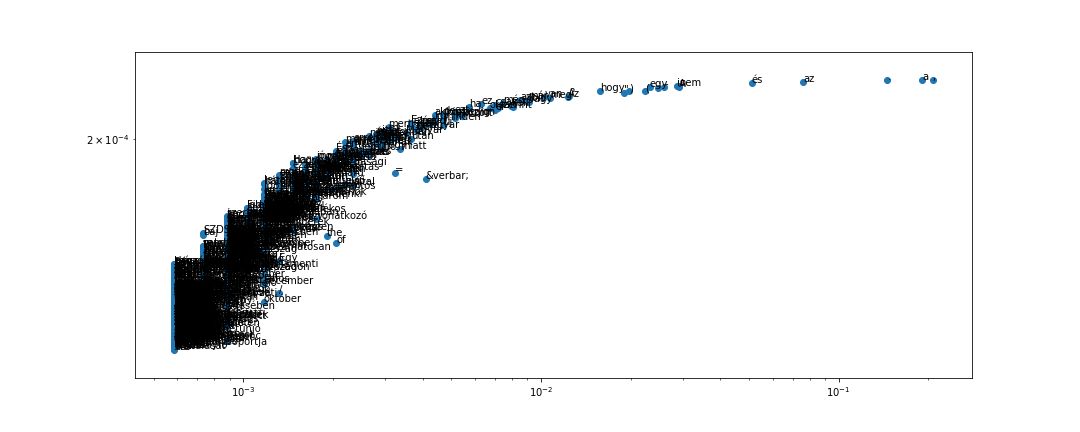
\includegraphics[width=\columnwidth]{current-flow-closeness.png}
                  %\caption{A szavak eloszlása \emph{closeness centrality} szerint.}
            \end{center}
                \label{fig:closeness}
          \end{figure}
        \end{block}

        \begin{block}{HITS}
          \begin{figure}[h]
            \begin{center}
              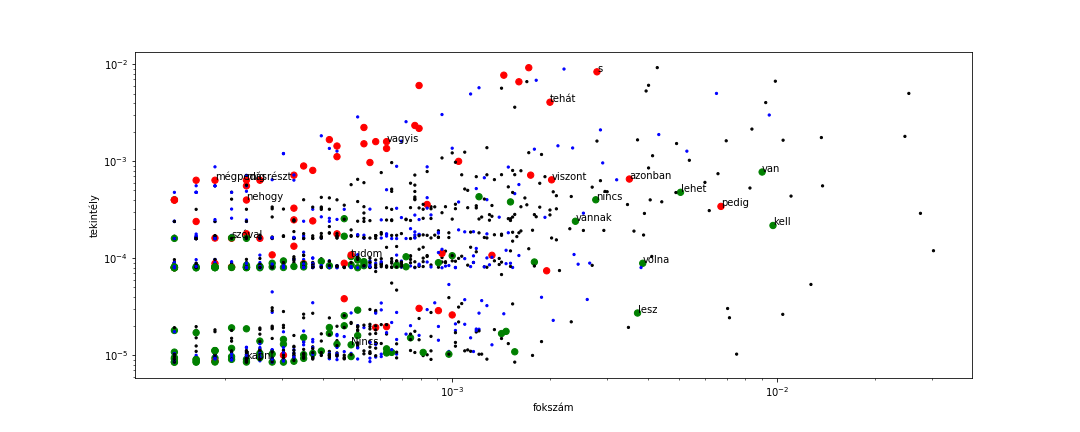
\includegraphics[width=\columnwidth]{conj-verb-auth.png}
                  \caption{%A HITS algoritmus eredménye.
                  A nagyobb piros ponttal jelölt kötőszavak balra fent
                  (magasabb authority),
                  a nagyobb zöld ponttal jelölt igék jobbra lent
                  (alacsonyabb authority)
                  helyezkednek el
                  a fokszám (gyakoriság) vs authority grafikonon.}
            \end{center}
                \label{fig:hits-auth}
          \end{figure}
            \begin{center}
            \url{https://github.com/makrai/textBetweenness}
            \end{center}
        \end{block}
      \end{column}

    \begin{column}{\sepwid} \end{column}			% empty spacer column

      \begin{column}{\onecolwid} % jobb oszlop
        \begin{block}{Központiság}
          \begin{figure}
            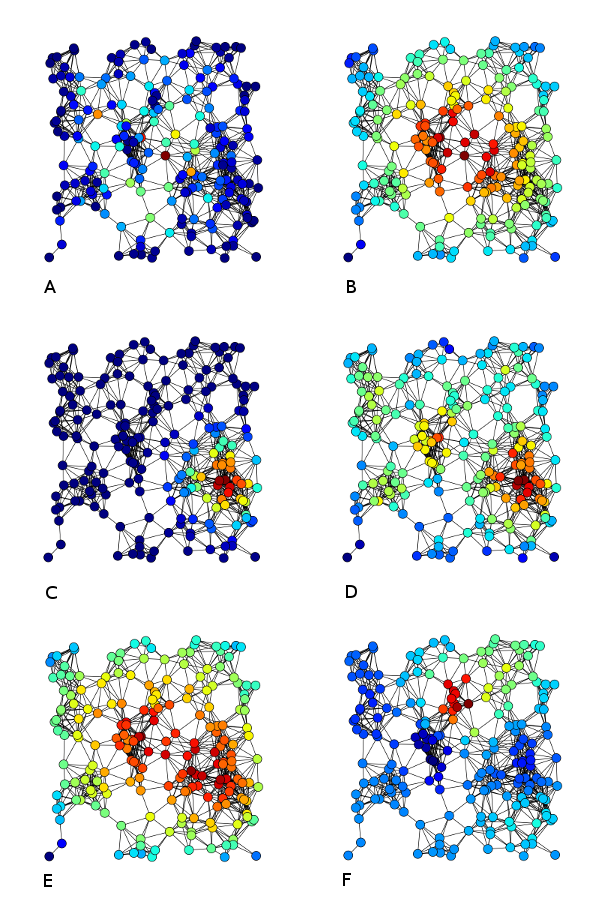
\includegraphics{6_centrality_measures}
            \begin{itemize}
              \item[A] köztiség (betweenness),
              \item[B] közelség (closeness),
              \item[C] sajátvektor-,
              \item[D] fok,
              \item[E] harmonikus,
              \item[F] Katz
            \end{itemize}
          \end{figure}
        \end{block}


        \begin{block}{További kutatás}
          \begin{itemize}
            \item az élsúlyok alkalmas skálázása
            \item kéne egy olyan szoftvercsomag, ami hatékonyan kezel
              irányított gráfokat
            \item klikkek szófajok szerint?
            \item szemantika
          \end{itemize}
        \end{block}

        \begin{block}{Hivatkozások}
          \small
          %\footnotesize
          \bibliographystyle{abbrvnat}
          \bibliography{minden}
        \end{block}

      \end{column}
  \end{columns}
\end{frame}
\end{document}

